
	
\chapter{Implementacija i korisničko sučelje}
		
		
		\section{Korištene tehnologije i alati}

		Komunikacija našem u timu je realizirana korištenjem aplikacija Discord\footnote{https://discord.com/} i Whatsapp\footnote{https://www.whatsapp.com/}.\\ Za izradu UML dijagrama korišten je alat Astah Professional\footnote{http://astah.net/editions/professional}, a kao sustav za upravljanje
izvornim kodom Git\footnote{https://git-scm.com/}. Udaljeni repozitorij projekta je dostupan na web platformi GitLab\footnote{https://gitlab.com/}, a kao razvojno okruženje korišten je IntelliJ IDEA\footnote{https://www.jetbrains.com/idea/} - tvrtke JetBrains\footnote{https://www.jetbrains.com/} te Microsoftov Visual Studio Code\footnote{https://visualstudio.microsoft.com/
}. 
	\\
	 Naša aplikacija napisana je koristeći Spring Framework\footnote{https://spring.io/} i jezik Java\footnote{https://www.oracle.com/java/} za izradu backenda te React\footnote{https://reactjs.org/} - JavaScript library za izradu frontenda. React je open-source, front end, JavaScript knjižnica za izgradnju korisničkog sučelja ili UI komponenti. Održavaju ga Facebook i zajednica pojedinačnih programera i tvrtki. Spring razvojno okruženje je Java platforma koja pruža široki panel opcija kao podrški
razvoju Java aplikacija. Spring rukuje infrastrukturom, tako da programer može usmjeriti svoj
fokus na razvoj aplikacije. \\
Tijekom izrađivanja aplikacije koristili smo i Postman\footnote{https://www.postman.com/} za simuliranje HTTP zahtjeva nad aplikacijom, Google Drive\footnote{https://workspace.google.com/products/drive/} za efikasno dijeljenje organizacijskih informacija i raznih datoteka. 
Baza podataka se nalazi na poslužitelju u oblaku Amazon
Web Services\footnote{https://aws.amazon.com/}.			
			
			\eject 
		
	
		\section{Ispitivanje programskog rješenja}
			
			\textbf{\textit{dio 2. revizije}}\\
			
			 \textit{U ovom poglavlju je potrebno opisati provedbu ispitivanja implementiranih funkcionalnosti na razini komponenti i na razini cijelog sustava s prikazom odabranih ispitnih slučajeva. Studenti trebaju ispitati temeljnu funkcionalnost i rubne uvjete.}
	
			
			\subsection{Ispitivanje komponenti}

			\textbf{Unit testovi za Service sloj}
			\bigskip
			\newline
			Da bi napravili unit testove za svaki razred posebno, koristiti ćemo framework Mockito. Koristiti ćemo ga tako da "simuliramo" rad objekata koji testni razred koristi. @RunWith(MockitoJUnitRunner.class) je anotacija koja se stavlja iznad razreda u kojem su unit testovi. @InjectMocks anotacija nam označuje objekt nad kojim će se vršiti unit test (System under test). @Mock anotacija stvara objekt koji je "lažan", on neće izvoditi svoje normalne metode, već ćemo mu mi kako će se ponašati na svaki poziv metode.
			\bigskip
			\bigskip
			
			\bigskip
			\textbf{UserServiceJpa unit test}
			\bigskip
			
			\textit{listAll()} - metoda listAll() vraća listu korisnika (List<User>). U unit testu stvaramo 3 nova korisnika i simuliramo metodu listAll() da kao rezultat vrati listu od ta 3 korisnika. Zatim pozovemo metodu listAll() i provjerimo vraća li ta metoda dobre podatke nazad.
			
			\textit{registerUser()} - unit testovi za ovu metodu ispituju baca li IllegalArgumentException kada mu predamo korisnika kojemu fali neki od obaveznih podataka za registraciju ili kada već postoji korisnik s tim korisničkim imenom, emailom ili brojem telefona. Ispituje se i radi li metoda sve dobro kada mu predamo korisnika koji ima sve podatke, i ne postoje već korisnici s takvim korisničkim imenom, emailom i brojem telefona.
			
			\textit{updateUser()} - unit testovi za ovu metodu ispituju baca li IllegalArgumentException kada mu predamo korisnika kojemu fali neki od obaveznih podataka za ažuriranje podataka. Ispituje se i radi li metoda očekivano kada se preda korisnik kojemu bi se trebalo bez greške ažurirati podatke.
			
			\textit{findByUsername()} - unit testovi za ovu metodu ispituju baca li IllegalArgumentException kada mu predamo korisničko ime koje je null, vraća li null kada mu predamo korisničko ime za kojeg ne postoji registrirani korisnik i radi li metoda očekivano kada se preda korisničko ime za kojeg postoji registrirani korisnik.
			
			\textit{deleteUser()} - unit testovi za ovu metodu ispituju vraća li ispravno broj obrisanih korisnika. Ukoliko mu predamo korisničko ime za koje ne postoji registrirani korisnik treba vraćati da je broj obrisanih korisnika 0, a ako mu predamo korisničko ime za koje postoji registrirani korisnik treba vraćati da je broj obrisanih korisnika 1.
			
			\textit{getStatistics()} - Ukoliko ne postoje registrirani korisnici pri pozivu ove metode, ona bi trebala vratiti praznu listu. Ako postoje registrirani korisnici, ali ne njih više od dva, metoda bi trebala vratiti samo listu od tog jednog ili dva korisnika, tako da je prvi onaj bolje ocjenjeni. Ako postoji tri ili više registriranih korisnika metoda bi trebala vratiti listu od tri najbolje ocjenjena korisnika. Testira se i u kojem poretku je metoda vratila najbolje ocijenjene korisnike, tu se testira je li dobro implementirano sortiranje korisnika.
			
			\bigskip
			\bigskip
			\textbf{RatingServiceJpa unit test}
			\bigskip
			
			\textit{calculateAverageRatingForUser()} - Ukoliko se preda korisnik čije korisničko ime nema registrirano u bazi podataka baca se NonexistingUserReferencedException. Ako postoji korisnik, ali nema nikakvih ocjena za njega, metoda bi trebala vratiti ocjenu 0.0 . Testira se i računa li metoda ispravno prosječnu ocjenu za korisnika koji postoji i za kojega ima više ocjena spremljenih u bazi.
			
			\bigskip
			\bigskip
			\textbf{RequestServiceJpa unit test}
			\bigskip
			
			\textit{addRequest()} - Ako se metodi preda zahtjev čiji je autor postavljen na null, metoda bi trebala postaviti ulogiranog korisnika kao autora zahtjeva. Ako adresa zahtjeva ne sadrži opis, x kordinatu ili y kordinatu, metoda bi trebala baciti IllegalArgumentException. Ako je predan zahtjev koji je potpun i točan metoda bi trebala uspješno dodati zahtjev.
			
			\bigskip
			\begin{figure}[H]
				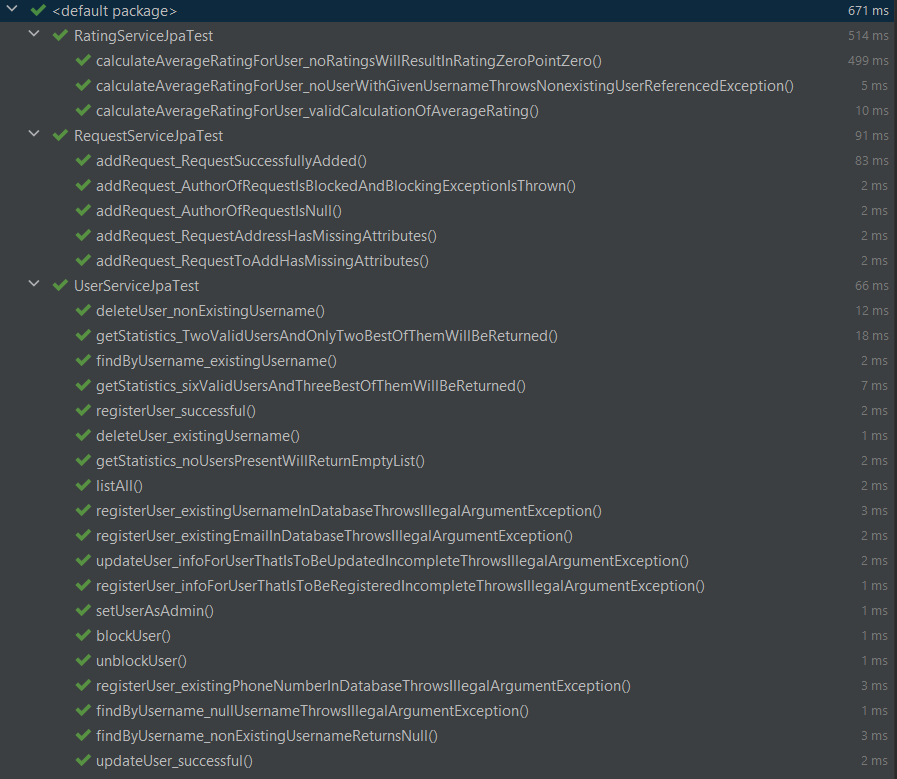
\includegraphics[scale=0.8]{slike/unit_testovi.png}
				\centering
				\caption{Rezultati unit testova}
				
			\end{figure}
			
			
			\subsection{Ispitivanje sustava}
			
			 \textit{Potrebno je provesti i opisati ispitivanje sustava koristeći radni okvir Selenium\footnote{\url{https://www.seleniumhq.org/}}. Razraditi \textbf{minimalno 4 ispitna slučaja} u kojima će se ispitati redovni slučajevi, rubni uvjeti te poziv funkcionalnosti koja nije implementirana/izaziva pogrešku kako bi se vidjelo na koji način sustav reagira kada nešto nije u potpunosti ostvareno. Ispitni slučaj se treba sastojati od ulaza (npr. korisničko ime i lozinka), očekivanog izlaza ili rezultata, koraka ispitivanja i dobivenog izlaza ili rezultata.\\ }
			 
			 \textit{Izradu ispitnih slučajeva pomoću radnog okvira Selenium moguće je provesti pomoću jednog od sljedeća dva alata:}
			 \begin{itemize}
			 	\item \textit{dodatak za preglednik \textbf{Selenium IDE} - snimanje korisnikovih akcija radi automatskog ponavljanja ispita	}
			 	\item \textit{\textbf{Selenium WebDriver} - podrška za pisanje ispita u jezicima Java, C\#, PHP koristeći posebno programsko sučelje.}
			 \end{itemize}
		 	\textit{Detalji o korištenju alata Selenium bit će prikazani na posebnom predavanju tijekom semestra.}
			
			\eject 
		
		
		\section{Dijagram razmještaja}
			
			Na slici 5.1 nalazi se dijagram razmještaja koji prikazuje raspored programske podrške aplikaciji unutar sklopovlja.
			
			Sa strane korisnika aplikacije, sklopovlje predstavlja njegovo računalo, mobilni telefon ili bilo koji drugi uređaj s pristupom internetu i instaliranim browserom.
			Internetski browser zadužen je za uspostavu konekcije sa poslužiteljem koja će omogućiti slanje i posluživanje zahtjeva.
			Sa strane poslužitelja sklopovlje predstavlja serversko računalo.
			Dvije glavne usluge koje se nalaze na serverskom računalu su baza podataka i web server koje su nužne za posluživanje zahtjeva.
			
			Komunikacija između korisnika i poslužitelja vrši se putem \textit{stateless} HTTP protokola. 
			Tijekom slanja zahtjeva serveru, korisnikov browser ima otvorenu jednu HTTP vezu prema serveru.
			S druge strane server može posluživati više zahtjeva iz više različitih izvora te stoga može imati i više aktivnih HTTP veza.
			
			\begin{figure}[h]
				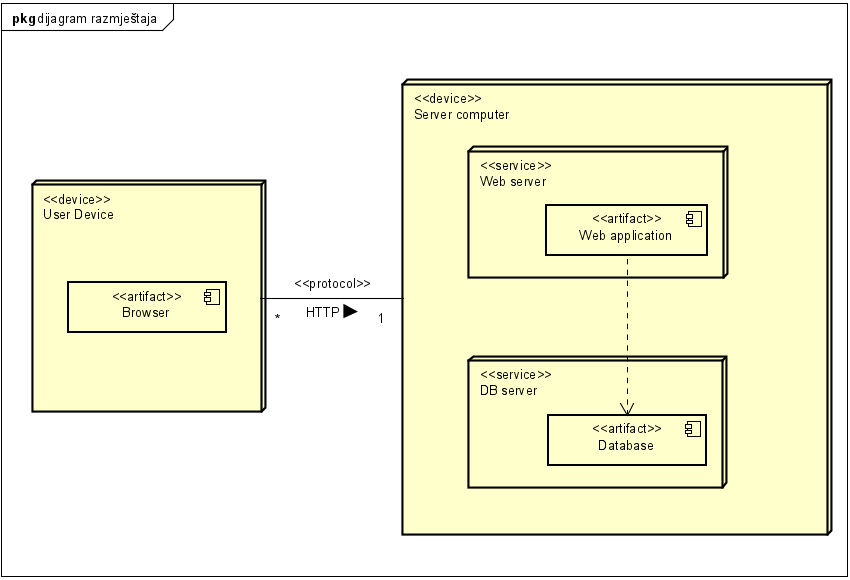
\includegraphics[height=0.5\textheight]{dijagramRazmjestaja}
				\caption{Dijagram razmještaja}
			\end{figure} 
			
			\eject 
		
		\section{Upute za puštanje u pogon}
		
			Grupa TODO odlučila se pokoriti našim Amazonskim overlordima i aplikaciju pustiti u pogon koristeći Amazon Web Services (AWS). Za korištenje AWS-a potrebno se registrirati i ostaviti podatke za plaćanje, koristimo besplatne mogućnosti dostupnih usluga te ništa neće biti naplaćeno. 
			
			Korisnik nakon registracije, odlazi na adresu \url{https://us-east-2.console.aws.amazon.com/console/home}, gdje dobiva prikaz dostupnih usluga:
			
			\begin{figure}[h]
				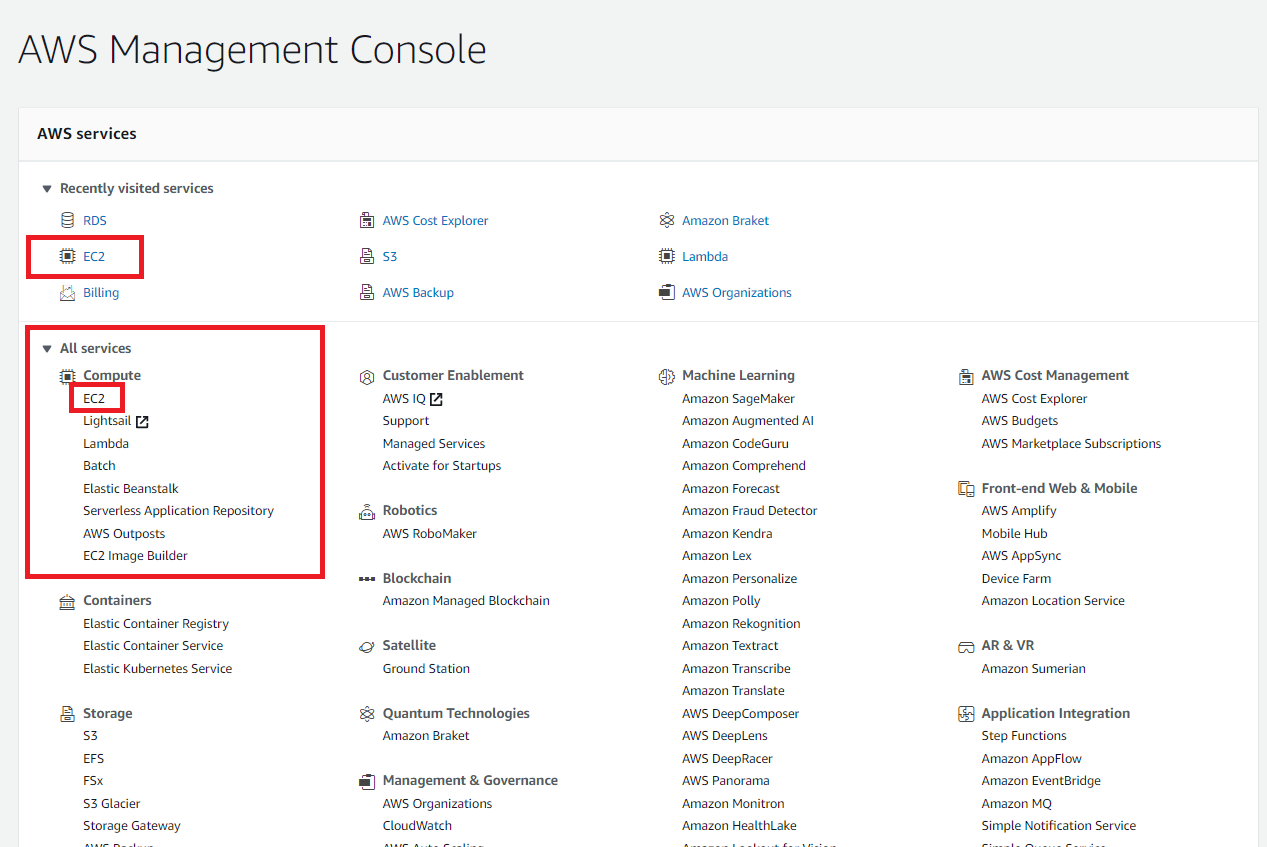
\includegraphics[scale=0.5]{slike/deployment_slike/awshome.png}
				\centering
				\caption{Dostupne AWS usluge}
				
			\end{figure}
		
			Biramo link EC2  koji nas vodi na iduću stranicu,gdje želimo stisnuti na pokretanje nove instance virtualnog stroja (Slika 5.4), potom odabiremo operacijski sustav virtualnog stroja(Slika 5.5). Biramo OS sa slike zato što je dostupan za besplatno korištenje. U idućem koraku ponovo odabiremo besplatan tip instance (Slika 5.6), klikamo Review and Launch i Launch, postavljamo i preuzimamo ključ za pristup instanci (neće biti potreban, al ga je dobro pričuvat). Posljednji put pritišćemo Launch i pokreće se instanciranje virtualnog stroja. Zatim na adresi \url{https://us-east-2.console.aws.amazon.com/ec2/v2/home} možemo pregledati vlastite instance virtualnih strojeva (Slika 5.7). Na "running" instancu desni klik i Connect. Možemo birati više načina spajanja, biramo treću opciju zbog jednostavnosti i pritišćemo gumb Connect (Slika 5.8). Otvara nam se linux terminal u browseru (Slika 5.9) i možemo krenuti s konfiguracijom virtualnog stroja.
			
			
			\noindent Prvo unosimo naredbu:
			\begin{center}
				\$ sudo yum update
			\end{center}
				kako bi primjenili ažuriranja. Za uspješno puštanje u pogon potrebni su nam Java, Git i Maven. Njih ćemo instalirati redom upisujući naredbe
				\begin{center}
					\$ sudo yum install java-11
				\end{center}
			\begin{center}
				\$ sudo yum alternatives  \texttt{--}config java
			\end{center}
			otvara nam se izbornik te odabiremo željenu verziju jave (Java 11 Amazon Corretto) unosom rednog broja pored imena verzije.
			Maven instaliravamo sljedećim nizom naredbi:
			\begin{center}
				\$ sudo wget http://repos.fedorapeople.org/repos/dchen/apache-maven/epel-apache-maven.repo -O /etc/yum.repos.d/epel-apache-maven.repo
				
				\$ sudo sed -i s/$\backslash$\$releasever/6/g /etc/yum.repos.d/epel-apache-maven.repo
				
				\$ sudo yum install -y apache-maven
			
				\$ mvn --version
			\end{center}
			Dalje, unosimo naredbe:
			\begin{center}
				\$ sudo yum install git -y
				
				\$ git clone \{adresa repozitorija\}
			\end{center}
			Nakon toga potrebno se pozicionirati u direktorij izvornog koda (onaj gdje se nalazi pom.xml), i pokrenuti instalaciju naredbom:
			\begin{center}
				\$ mvn clean install
			\end{center}
			Nakon instalacije, u direktoriju /targer nalazi se .jar datoteka koja predstavlja našu izgrađenu aplikaciju. Aplikaciju pokrećemo izvođenjem sljedeće naredbe:
			\begin{center}
				\$ nohup java -jar \{ime aplikacije\}.jar
			\end{center}
			Aplikacija je nakon nekoliko trenutaka pokrenuta i moguće joj je pristupiti preko javne adrese instance, na portu 8080, ali tek nakon što u AWS konzoli podesimo parametre sigurnosti, upute za to ostavljamo da korisnik sam prouči: \url{https://docs.aws.amazon.com/AWSEC2/latest/UserGuide/ec2-security-groups.html}
		
		
		
			
			\begin{figure}[h]
				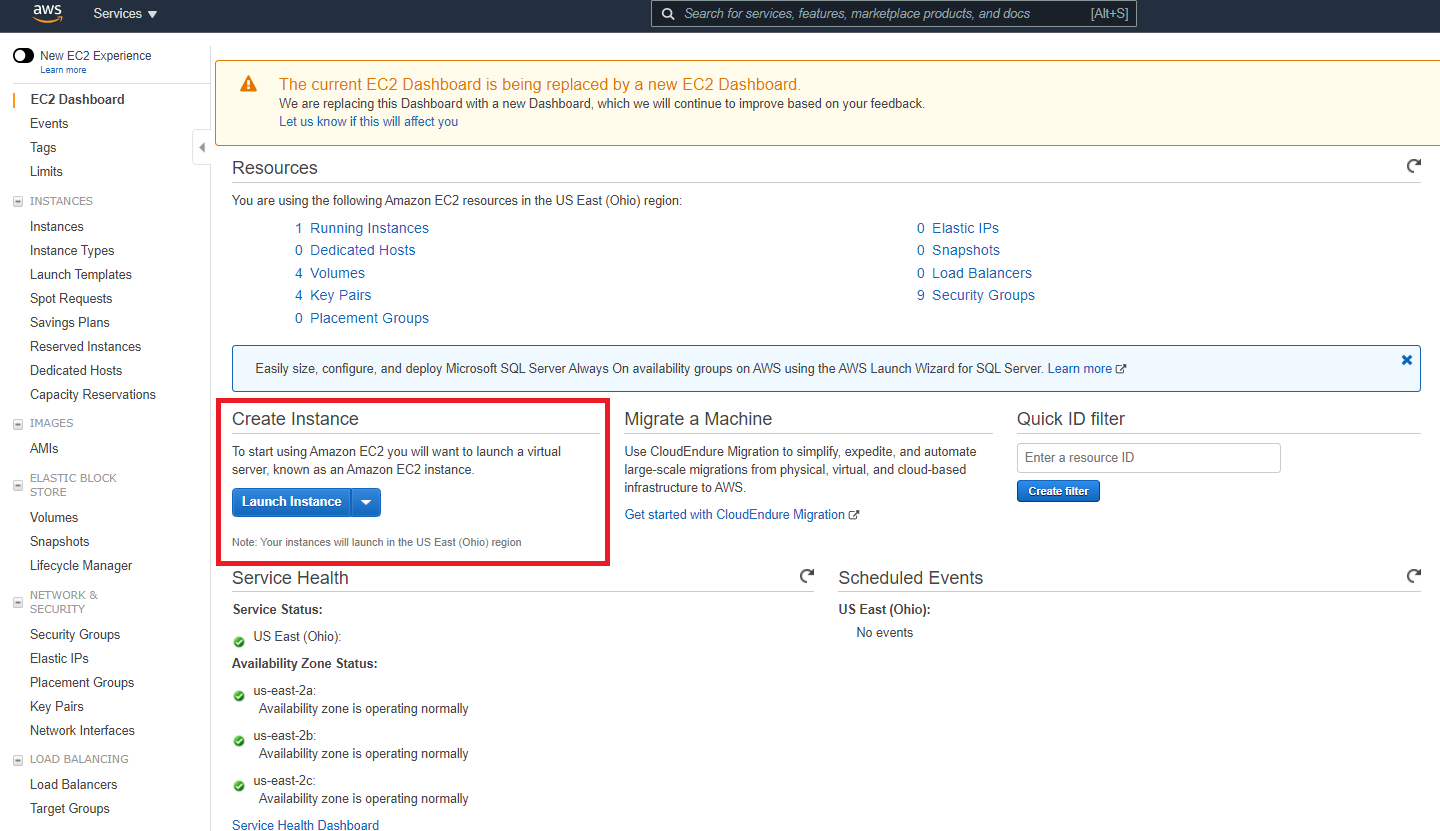
\includegraphics[width=\textwidth]{slike/deployment_slike/launchingInstance.png}
				\centering
				\caption{Pokretanje inicijalizacije}
			\end{figure}
		
			\begin{figure}[h]
				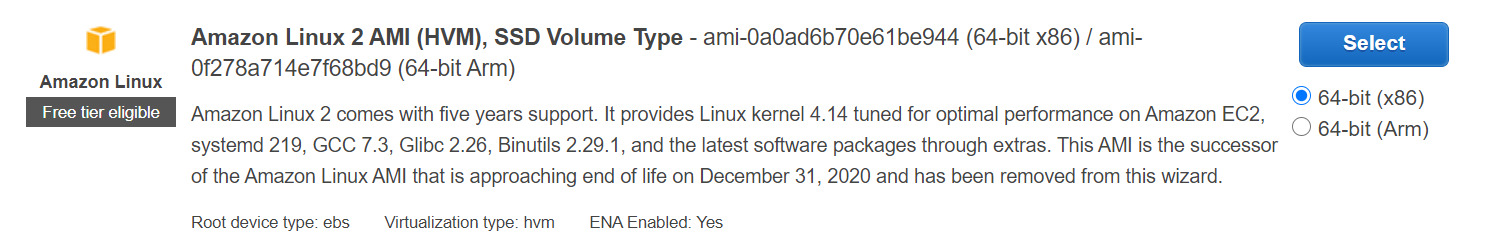
\includegraphics[width=\textwidth]{slike/deployment_slike/virtualOS.png}
				\centering
				\caption{Odabrani OS}
			\end{figure}
		
			\begin{figure}[h]
				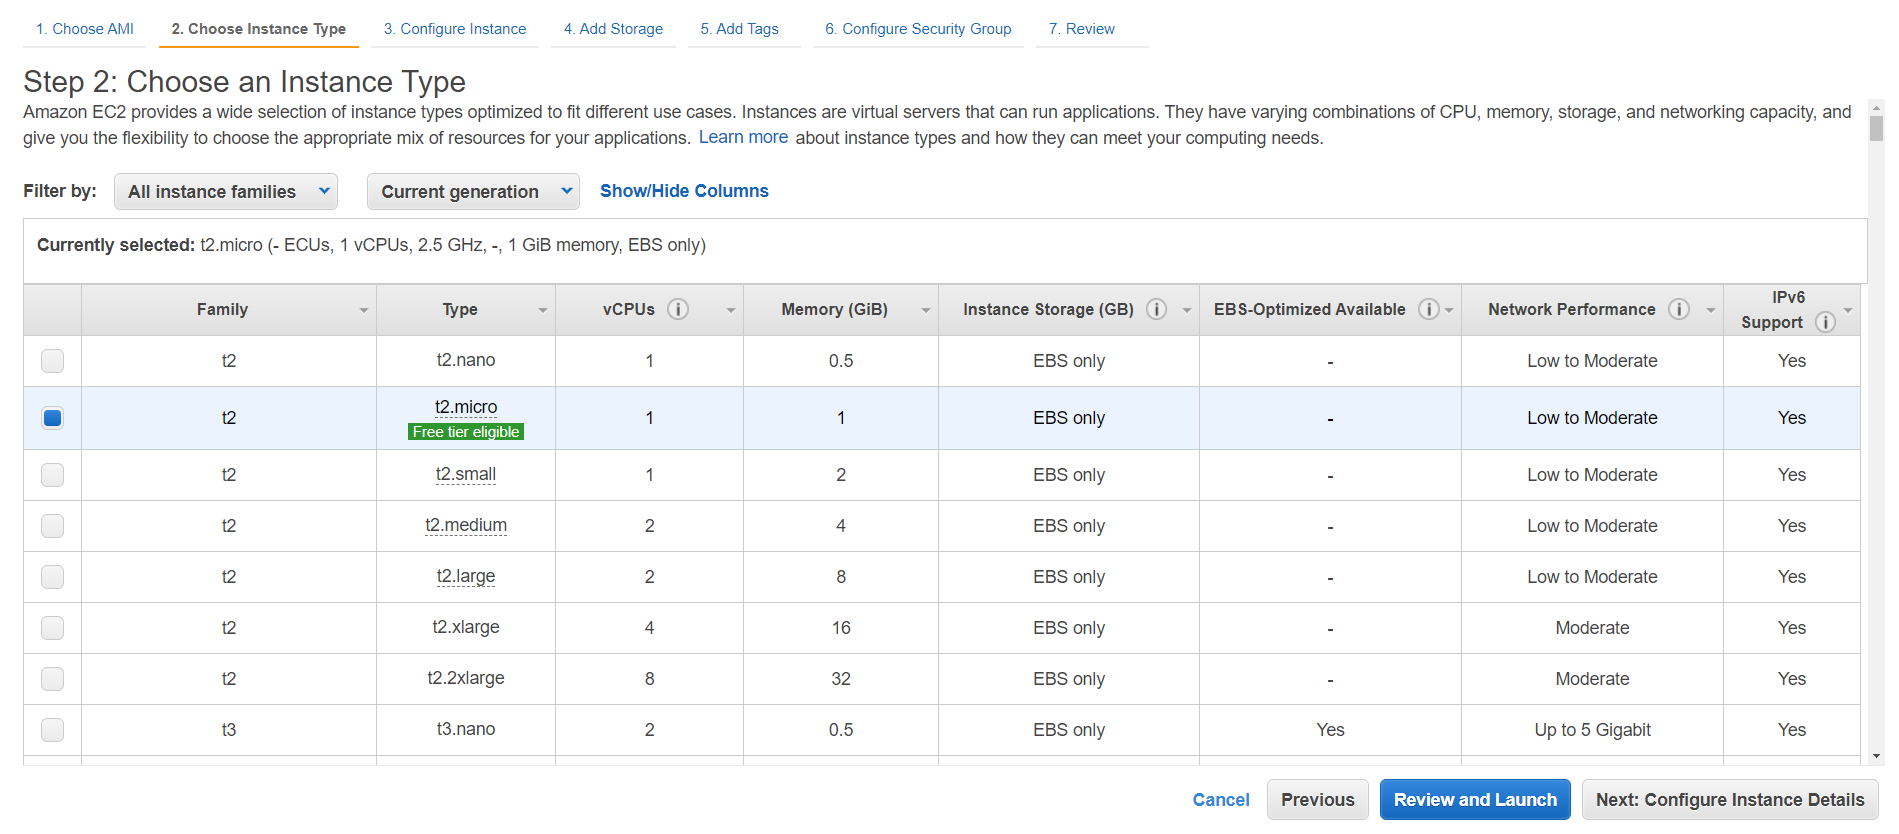
\includegraphics[width=\textwidth]{slike/deployment_slike/instanceType.png}
				\centering
				\caption{Tip instance}
			\end{figure}
			
			\begin{figure}[h]
				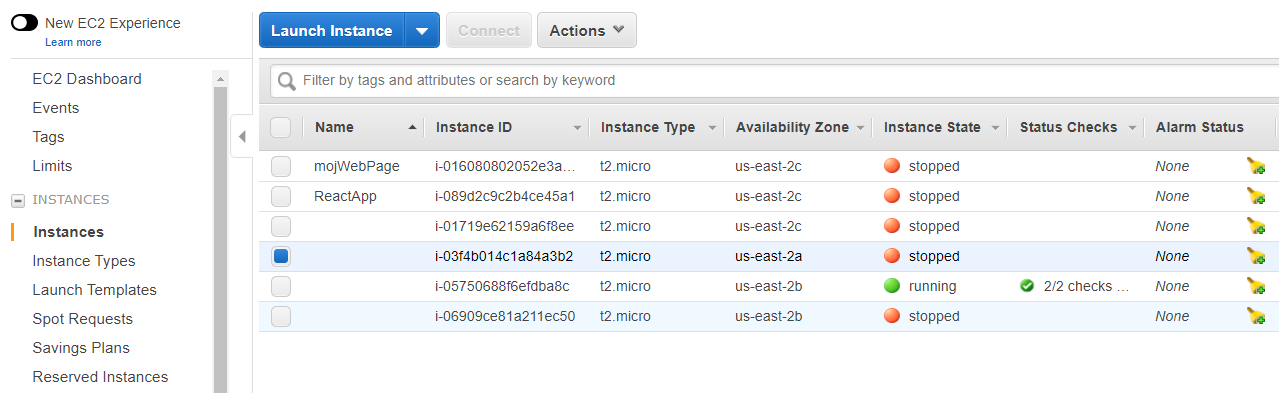
\includegraphics[width=\textwidth]{slike/deployment_slike/mojeInstance.png}
				\centering
				\caption{Instance}
			\end{figure}
			
			\begin{figure}[h]
				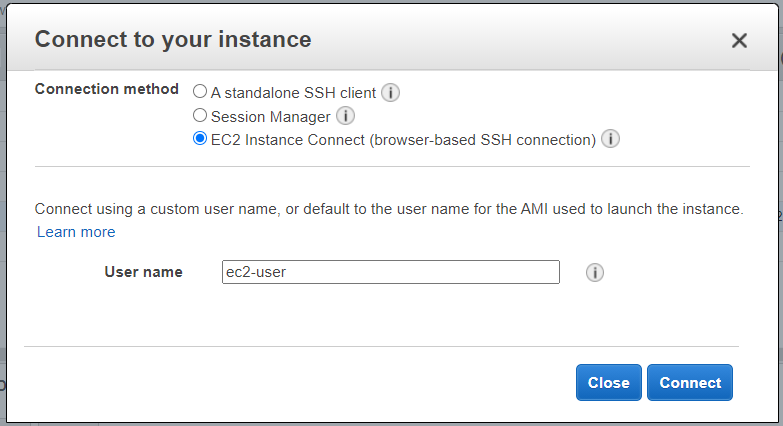
\includegraphics[width=\textwidth]{slike/deployment_slike/instanceConnect.png}
				\centering
				\caption{Spajanje na virtualni stroj}
			\end{figure}
		
			\begin{figure}[h]
				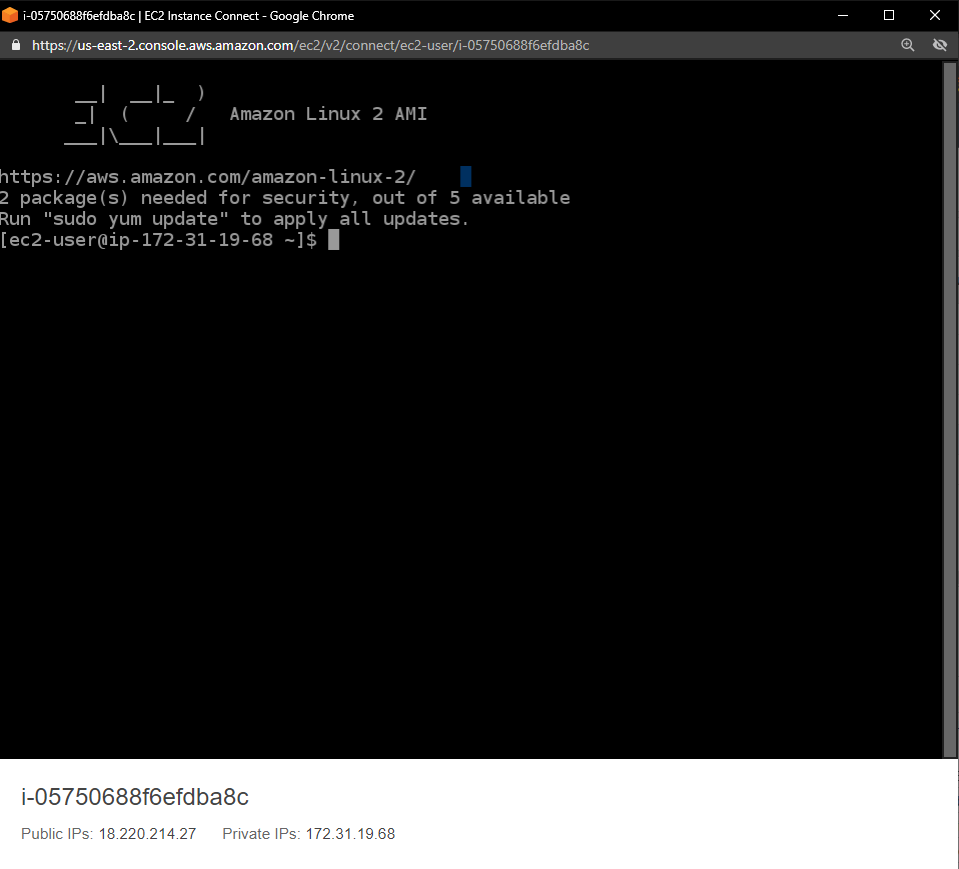
\includegraphics[width=\textwidth]{slike/deployment_slike/browserTerminal.png}
				\centering
				\caption{Browser terminal}
			\end{figure}
			
			\eject 